\documentclass[14p]{report}
\usepackage{amsfonts}
\usepackage{amsmath}
\usepackage{yfonts}
\usepackage{mathrsfs}
\usepackage{amssymb}
\usepackage[T1]{fontenc}
\usepackage{pgfplots}
\usepackage[margin=1in]{geometry}
\usepackage{xcolor}
\usepackage{pgfplotstable}
\pgfplotsset{compat=newest}

\title{Lineáris regresszió elméleti összefoglaló}
\author{Bognár Miklós}
\date{Bevezetés az Ökonometriába}

\pagecolor{white}
\color{black}

\def\pmb{\boldsymbol}
\def\ebeta{\hat{\pmb{\beta}}}
\def\e{\epsilon}
\def\bar{\overline}

\selectcolormodel{gray}

\makeatletter
\pgfdeclareplotmark{dot}
{%
	\fill circle [x radius=0.02, y radius=0.08];
}%
\makeatother

\begin{document}
	\maketitle
	\tableofcontents
	\newpage
	\section{Matematikai összefoglaló}
	A lineáris regresszió megértéséhez elengedhetetlen, hogy tisztában legyünk néhány, lineáris algebrából ismeretes fogalommal és összefüggéssel. Ezen felül nagyon hasznos, ha ismerjük, hogy hogyan kezelendőek a valószínűségi vektorváltozók illetve a mártixdifferenciálás-kifejezések.  
	
	\subsection{Pszeudoinverzek}
	Legyen $\pmb{A} \in \mathbb{R}^{n\times m}, n \ne m$ nem négyzetes mátrix. Ha egy  $\pmb{A}x = y , x \in \mathbb{R}^{m\times 1}, y \in \mathbb{R}^{n \times 1}$ lineáris egyenletrendszer együtthatómátrixaként gondolunk rá, akkor $n \ge m$ vagy $m \ge n$ esetén rendre a \emph{túlhatározottság} vagy \emph{alulhatározottság} esete állna fent, az első esetben általánosságban nem lenne megoldásunk, a második esetben pedig végtelen sok megoldásunk lenne rá. Látszik, hogy az $n \ne m$ esetben nem beszélhetünk $\pmb{A}^{-1}$ inverzről, helyette egy általánosabb, úgynevezett \emph{pszeudoinverz} kell.
	\\
	\\
	Egy $\pmb{A} \in \mathbb{R}^{n \times m}, n > m$ mátrix \emph{bal oldali pszeudoinverze} (Más néven \emph{Moore-Penrose pszeudoinverz}):
	\[
	\pmb{A}^{\dagger} := (\pmb{A}^T\pmb{A})^{-1}\pmb{A}^T \in \mathbb{R}^{m \times n}
	\]
	Figyeljük meg, hogy ha $\pmb{A}^{\dagger}$-el balról megszorozzuk $\pmb{A}$-t, az identitás mátrixot kapjuk, tehát bal oldalról valóban identitásként működik:
	\[
	\pmb{A}^{\dagger}\pmb{A} = (\pmb{A}^T\pmb{A})^{-1}\pmb{A}^T\pmb{A} = \pmb{I}
	\]
	Ha jobbról szoroznánk meg:
	\[
	\pmb{A}\pmb{A}^{\dagger} = \pmb{A}(\pmb{A}^T\pmb{A})^{-1}\pmb{A}^T
	\]
	Ez semmi más, mint a \emph{projekció-mátrix} $\pmb{A}$ oszlopvektorai által kifeszített vektortérre. Ha egy vektor ebben az oszloptérben van, rá persze identitásként hat $\pmb{A}\pmb{A}^{\dagger}$, ha viszont ezen kívül esik, akkor rávetíti az oszloptérre a vektort. Egy túlhatározott $\pmb{A}x = y$ egyenletrendszert tehát "meg lehet oldani", ha $y$-t rávetítjük $\pmb{A}$ oszlopterére, és megoldjuk az $\pmb{A}x = \tilde{y}$ egyenletrendszert: 
	\[
	\tilde{y} = \pmb{A}(\pmb{A}^T\pmb{A})^{-1}\pmb{A}^T y = \pmb{A}\pmb{A}^{\dagger} y
	\]
	\[
	\pmb{A}x = \tilde{y} = \pmb{A}\pmb{A}^{\dagger}y
	\]
	\[
	\pmb{A}^{\dagger}\pmb{A}x = \pmb{A}^{\dagger}\pmb{A}\pmb{A}^{\dagger}y
	\]
	\[
	x  = \pmb{A}^{\dagger}y
	\]
	
	Az $n < m$ esetben alulhatározottság áll fenn, itt \emph{jobb oldali pszeudoinverzről} beszélhetünk:
	\[
	\pmb{A}^{\ddagger} := \pmb{A}^T(\pmb{A}\pmb{A}^T)^{-1} \in \mathbb{R}^{n \times m}
	\]
	Bár ezt nem fogjuk a későbbiekben használni, érdemes lehet megjegyezni, hogy a jobb oldali pszeudoinverzzel való balról szorzás esetén - hasonlóan a bal oldali pszeudoinverzhez - projekciómátrixot kapunk, csak most $\pmb{A}$ sorvektorai által kifeszített vektortérre.
	\subsection{Valószínűségi vektorváltozók}
	Egy $\pmb{\xi} = [\xi_1, \dots , \xi_n]^T$ vektort \emph{valószínűségi vektorváltozónak} hívunk, ha $\forall i$-re $\xi_i$ skalárértékű valószínűségi változó. A továbbiakban csak a vektorértékű normális eloszlást követő valószínűségi vektorváltozókkal foglalkozunk, ezek formálisan felírva:
	\[
	\pmb{\xi} \sim \mathcal{N}(\pmb{\mu}, \pmb{\Sigma})
	\]
	ahol $\pmb{\mu} \in \mathbb{R}^{n \times 1}$ a várható értékek vektora, $\pmb{\Sigma}$ pedig a \emph{variancia-kovarianca mátrix}. Természetesen $Var[\pmb{\xi}] = \pmb{\Sigma}$. Természetesen $\pmb{\Sigma} \in \mathbb{R}^{n \times n}$ pozitív szemidefinit és szimmetrikus mártix. Az $n = 1$ esettel analóg módon $\pmb{\xi}$ sűrűségfüggvénye
	\[
	f_{\pmb{\xi}}(\xi_1, \dots, \xi_n) = \frac{ e^{-\frac{1}{2}(\pmb{\xi}-\pmb{\mu})^T\pmb{\Sigma}^{-1}(\pmb{\xi}-\pmb{\mu})}}{\sqrt{(2\pi)^n|\pmb{\Sigma}|}}
	\]
	A sűrűségfüggvény $n = 2$ esetben $\pmb{\mu} = [2, -1]^T$ és $\pmb{\Sigma} = \pmb{I}$ várhatóérték és kovariancia mátrix mellett: 
	\def\centerx{2}
	\def\centery{-1}
	
	\begin{center}
		\begin{tikzpicture}
			\begin{axis}
				\addplot3[surf,domain=-2:6,domain y=-5:3] 
				{exp(-( (x-\centerx)^2 + (y-\centery)^2)/3 )};
				\node[circle,inner sep=1pt,fill=blue,pin=90:$\pmb{\mu}$] 
				at (axis cs:\centerx,\centery,1) {};
			\end{axis}
		\end{tikzpicture}
	\end{center} 
	Egy $\pmb{A} \in \mathbb{R}^{n \times n}$ mátrix mellett a skaláresethez hasonlóan 
	\[
	Var[\pmb{A}\pmb{\xi}] = \pmb{A} \pmb{\Sigma} \pmb{A}^T
	\]
	\[
	\mathbb{E}[\pmb{A}\pmb{\xi}] = \pmb{A}\mathbb{E}[\pmb{\xi}]
	\]
	$\pmb{\Sigma}$ kovariancia mátrixot kifejezhetjük várható értékekkel is:
	\[
	\pmb{\Sigma} = \mathbb{E}[(\pmb{\xi}-\mathbb{E}[\pmb{\xi}])(\pmb{\xi}-\mathbb{E}[\pmb{\xi}])^T] = \mathbb{E}[\pmb{\xi}\pmb{\xi}^T] - \mathbb{E}[\pmb{\xi}]\mathbb{E}[\pmb{\xi}^T]
	\]
	$\pmb{\Sigma}$ alakja:
	\[
	\pmb{\Sigma} = 
	\begin{bmatrix}
		\sigma_1^2 & Cov[\xi_1,\xi_2] & \dots & Cov[\xi_1,\xi_n] \\
		Cov[\xi_2,\xi_1] & \sigma_2^2 & \dots & Cov[\xi_2,\xi_n] \\
		\vdots & \vdots & \ddots & \vdots \\
		Cov[\xi_n,\xi_1] & Cov[\xi_n,\xi_2] & \dots & \sigma_n^2
	\end{bmatrix}
	\]
	ahol $\sigma_1^2, \dots, \sigma_n^2$ rendre $\xi_1, \dots, \xi_n$ varianciái.
	\subsection{Mátrixdifferenciálás nagyon röviden}
	Legyenek $\pmb{a}, \pmb{b} \in \mathbb{R}^{k \times 1}$ vektorok. Ekkor
	\[
	\frac{\partial\pmb{a}^T\pmb{b}}{\partial\pmb{b}} = \frac{\partial\pmb{b}^T\pmb{a}}{\partial\pmb{b}} = \pmb{a}
	\]
	Ha $\pmb{A} \in \mathbb{R}^{k \times k}$ mátrix, akkor
	\[
	\frac{\partial\pmb{b}^T\pmb{A}\pmb{b}}{\partial\pmb{b}} = 2\pmb{A}\pmb{b}
	\]
	Ha $\pmb{A}$ szimmetrikus, akkor ezen felül
	\[
	2\pmb{A}\pmb{b} = 2\pmb{b}^T\pmb{A}
	\]
	Legyen $\pmb{\beta} \in \mathbb{R}^{k \times 1}$, $\pmb{A} \in \mathbb{R}^{n \times k}$ és $\pmb{y} \in \mathbb{R}^{n \times 1}$. Ekkor
	\[
	\frac{\partial 2\pmb{\beta}^T\pmb{A}^T\pmb{y}}{\partial\pmb{\beta}} = \frac{\partial 2\pmb{\beta}^T(\pmb{A}^T\pmb{y})}{\partial\pmb{\beta}} = 2\pmb{A}^T\pmb{y}
	\]
	
	\section{A lineáris regresszió}
	A regresszió kiindulópontja egy $\mathscr{X}$ normális eloszlású sokaság, melynek minden tagja rendelkezik $\pmb{x}_i$ \emph{featurevektor}-ral, avagy magyarázó változó-vektorral (ezek a \emph{regresszorok}), illetve egy-egy skalár $y_i$ \emph{label}-lel, avagy magyarázott változóval (amiket a regresszorok magyaráznak egy lineáris modell alapján, ezt később jobban kifejtjük). A sokaságból $n$ darab mintát veszünk (megfigyelést végzünk), \emph{a minták iid. normális eloszlásúak}, ami persze azt jelenti, hogy \emph{minden magyarázó változó-vektor egy vektorértékű normális eloszlású valószínűségi vektorváltozó}. Létezik egy másik konstrukció is, miszerint $\pmb{X}$ rögzített, és nem változik mintavételről mintavételre, ez azonban csak annyit jelent, hogy mindenhol, ahol feltételes eloszlás/várható érték van, onnan az $\mid \pmb{X}$ feltételt ki kell venni. Mi $\pmb{X}$-re mint valószínűségi vektorváltozók mátrixa tekintünk mostantól.
	\\
	\\
	A megfigyelt magyarázó változó-vektorokat soronként egymásra rakva felépítünk egy úgynevezett \emph{design mátrix}ot, melyet mostantól $\pmb{X}$-el jelölünk. Minden $\pmb{x}_i$ magyarázó változó-vektor első eleme konstans $1$, ez tölti be az intercept, avagy kétdimenziós esetben az y-tengellyel való metszéspont szerepét. $n$ darab megfigyelés és $p$ elemszámú magyarázó változó-vektorral $\pmb{X}$ alakja a következő:
	\[
	\pmb{X} = 
	\begin{bmatrix}
		1 & x_{1,1} & \dots & x_{1,p-1} \\
		1 & x_{2,1} & \dots & x_{2,p-1} \\
		\vdots & \vdots & \ddots & \vdots \\
		1 & x_{n,1} & \dots & x_{n,p-1}	
	\end{bmatrix}_{n \times p}
	\]
	A megfigyelt magyarázott változókat szintén sorokba tömörítjük, így mivel mindegyik skalár, egy vektort kapunk:
	\[
	\pmb{y} =
	\begin{bmatrix}
		y_1 \\
		y_2 \\
		\vdots \\
		y_n
	\end{bmatrix}
	\]
	A lineáris regresszió kiindulópontja mindig egy \emph{modell}, avagy egy elméleti feltevés arról, hogy milyen kapcsolatban áll a magyarázott $\pmb{y}$ változó a magyarázó $\pmb{X}$ regresszorokkal.
	\[
	\pmb{y} = \pmb{X}\pmb{\beta} + \pmb{\epsilon}
	\]
	A lineáris kapcsolatot a $\pmb{\beta}$ együtthatóvektor (avagy \emph{paramétervektor}) írja le, míg $\pmb{\e}$ a regresszorok által nem magyarázott eltéréseket, avagy \emph{hibákat} jelenti. Mostantól $\pmb{\e}$-re \emph{hibavektor} néven hivatkozunk.
	\\
	\\
	A regresszió célja, hogy megtaláljuk azt a $\ebeta$ \emph{paraméterbecslés-vektort}, hogy az 
	\[
		\hat{\pmb{y}} = \pmb{X}\ebeta 
	\]
	úgynevezett \emph{predikciós} egyenletből származott \emph{becsült} $\hat{\pmb{y}}$ vektor a lehető legközelebb legyen a valódi megfigyelt $\pmb{y}$ vektorhoz.
	\\
	\\
	A lineáris regresszió egy darab regresszor (magyarázó változó) esetén az alábbi ábrával szemléltethető:
	
	\begin{center}
		\begin{tikzpicture}
			
			\begin{axis}[
				xmin = 0, xmax = 11,
				ymin = 0, ymax = 11,
				width = 0.5\textwidth,
				height = 0.35\textwidth,
				xtick distance = 1,
				ytick distance = 1,
				xlabel={$x$},
				ylabel={$y$},
				grid = both,
				minor tick num = 1,
				major grid style = {lightgray},
				minor grid style = {lightgray!25},
				]
				\addplot[teal, only marks] table[x = t, y = x] {regr-dat.dat};
				
				\addplot[
				thick,
				orange
				] table[
				x = t,
				y = {create col/linear regression={y=x}}
				] {regr-dat.dat};
				
				\addlegendentry{Adatpontok}
				\addlegendentry{
					Regresszió: $ \hat{y} =
					\pgfmathprintnumber{\pgfplotstableregressiona}
					\cdot x
					\pgfmathprintnumber[print sign]{\pgfplotstableregressionb}$
				};
				
			\end{axis}
		\end{tikzpicture}
	\end{center}
	Itt $\ebeta$ paraméterbecslés vektor alakja
	\[
	\ebeta = 
	\begin{bmatrix}
		\hat{\beta_0} \\
		\hat{\beta_1}
	\end{bmatrix}
	=
	\begin{bmatrix}
		1,87 \\
		0,69
	\end{bmatrix}
	\]
	Azt, hogy hogyan kaptuk meg $\ebeta$ paraméterbecslést, a következő fejezetek tárgyalják részletesen. Ezen kívül külön foglalkozunk majd a fenti egyváltozós regresszióval is (a $p=2$-es eset).
	
	\section{Az Ordinary Least Squares (OLS) becslési eljárás}
	A lineáris regresszió $\ebeta$-jának megtalálására az egyik lehetséges eljárás az Ordinary Least Squares, avagy legkisebb négyzetek módszere. Az eljárást kettő szemszögből is megvizsgáljuk.
	
	\subsection{Az OLS-becslés geometriai értelmezése}
	Szinte mindig $n > p$, azaz több megfigyelésünk van, mint amennyi magyarázó változónk, így az
	\[
		\pmb{X}\pmb{\beta} = \pmb{y}
	\]
	 egyenletrendszer \emph{túlhatározott}, és nagyon specifikus esetektől eltekintve nem létezik egzakt megoldás $\pmb{\beta}$-ra. Az első fejezetben azonban láttuk, hogy a bal oldali pszeudoinverz pontosan ezt a problémát orvosolja. A jelölési konvenció a megoldásból nyert \emph{paraméter-becslésre} $\ebeta$, ami a mintavétel véletlenszerűségéből adódóan maga is vektorértékű valószínűségi változó ($\ebeta$ pontos eloszlásáról a későbbiekben lesz szó):
	\[
	\ebeta = \pmb{X}^{\dagger}\pmb{y} = (\pmb{X}^T\pmb{X})^{-1}\pmb{X}^T\pmb{y}
	\]
	Ebben az esetben $\pmb{y}$-t az $\pmb{X}$ design mátrix oszlopterére vetítettük. $\pmb{X}^T\pmb{X}$ \emph{Gram-mátrix} néven is ismeretes (egyébként $\pmb{X}\pmb{X}^T$-ra is szoktak utalni ezen a néven, annyi különbséggel, hogy az előbbi a regresszorok közti korreláció mértékét mutatja a mintavételeken keresztülfutva, egyfajta \emph{temporális} módon, az utóbbi pedig magukon a regresszorokon keresztülfutva egyfajta \emph{térbeli} korrelációt mutat). Az $\pmb{X}^T\pmb{X}$ mátrix determinánsát \emph{Gram-determinánsnak} is hívják.
	\\
	\\
	Ha $n < p$, azaz kevesebb megfigyelésünk van, mint amennyi magyarázó változónk, az egyenletrendszer alulhatározott lesz, és nem fog létezni bal oldali pszeudoinverz, így nem lesz olyan $\pmb{X}^{\dagger}$ mátrix, amivel balról beszorozva $\pmb{X}$-et az identitásmátrixot kapnánk. Ha $\pmb{X}^{\ddagger}$-el próbálkozunk, ami létezik:
	\[
		\pmb{X}^{\ddagger}\pmb{X}\beta = \pmb{X}^{\ddagger}\pmb{y}
	\] 
	a bal oldalon $\pmb{X}$ sorterére való vetítési mátrixot kapnánk. Innen az is következik, hogy amint megtaláltuk $\ebeta$ első $n$ elemét, a maradék $p-n$ együttható az első $n$ együttható lineáris kombinációjaként állna elő szükségszerűen. Ezért mostantól feltesszük, hogy a "normális" $n > p$ eset áll fenn. 
	\\
	\\
	A továbbiakban a \emph{tényleges hibavektor} jelölése 
	$\pmb{e}$, a valós $y_i$-k és a $\pmb{X}\ebeta = \hat{\pmb{y}}$ modellbecslés által prediktált $\hat{y_i}$-k közti eltérések vektora (sokszor $\pmb{e}$-t $\widehat{\pmb{\e}}$-ként is jelölik):
	\[
	\pmb{e} =
	\begin{bmatrix}
		y_1 - \hat{y_1} \\
		y_2  - \hat{y_2} \\
		\vdots \\
		y_n - \hat{y_n}
	\end{bmatrix}
	\]
	\subsection{Az OLS-becslés mint szélsőérték-feladat}
	$\ebeta$ paraméterbecslés-vektort megkaphatjuk úgy is, ha tekintjük az alábbi minimalizálási feladatot:
	\[
	\pmb{e}^T\pmb{e} \rightarrow \min_{\ebeta}
	\]
	azaz minimalizáljuk a becsült $\hat{y}_i$ és tényleges $y_i$ magyarázott változók közötti négyzetösszeget. $\pmb{e}^T\pmb{e}$-t RSS, azaz \emph{sum of squared residuals} néven is emlegetik. Írjuk ki a hiba-négyzetösszeg teljes alakját:
	\[
	\pmb{e}^T\pmb{e} = (\pmb{y} - \pmb{X}\ebeta)^T(\pmb{y} - \pmb{X}\ebeta) = \pmb{y}^T\pmb{y} - \ebeta^T\pmb{X}^T\pmb{y} - \pmb{y}^T\pmb{X}\ebeta + \ebeta^T\pmb{X}^T\pmb{X}\ebeta = \pmb{y}^T\pmb{y} - 2\ebeta^T\pmb{X}^T\pmb{y} + \ebeta^T\pmb{X}^T\pmb{X}\ebeta
	\]
	Itt felhasználtuk, hogy a transzponálás "megfordítja a szorzatot", illetve hogy skalár transzponáltja önmaga, így $\pmb{y}^T\pmb{X}\ebeta = (\pmb{y}^T\pmb{X}\ebeta)^T = \ebeta^T\pmb{X}^T\pmb{y}$.
	A minimalizációhoz vennünk kell a kifejezés $\ebeta$ szerinti deriváltját, majd $0$-val egyenlővé tenni:
	\[
	\frac{\partial{\pmb{e}^T\pmb{e}}}{\partial\ebeta} = -2\pmb{X}^T\pmb{y} + 2\pmb{X}^T\pmb{X}\ebeta = 0
	\]
	Ebből megkapjuk az úgynevezett \emph{normálegyenletet}:
	\[
	(\pmb{X}^T\pmb{X})\ebeta = \pmb{X}^T\pmb{y}
	\]
	$(\pmb{X}^T\pmb{X})$ szimmetrikus, és ha feltesszük, hogy létezik inverze, akkor balról beszorozva mindét oldalt:
	\[
	(\pmb{X}^T\pmb{X})^{-1}(\pmb{X}^T\pmb{X})\ebeta = (\pmb{X}^T\pmb{X})^{-1}\pmb{X}^T\pmb{y}
	\]
	\[
	\ebeta = (\pmb{X}^T\pmb{X})^{-1}\pmb{X}^T\pmb{y}
	\]
	Látható, hogy pontosan ugyanaz jött ki, mint a pszeudoinverzes levezetésben. Míg ez utóbbi pusztán analitikus úton jutott el $\ebeta$-hoz, a pszeudoinverzes módszert geometrikus úton is el lehet képzelni.
	
	\section{Az OLS-becslés tulajdonságai}
	Vegyük az OLS paraméterbecslés normálegyenletét, és figyeljük meg, hogy $\pmb{X}^T\pmb{e} = \pmb{0}$:
	\[
	(\pmb{X}^T\pmb{X})\ebeta = \pmb{X}^T\pmb{y}
	\]
	A modellből adódóan $\pmb{y} = \pmb{X}\ebeta + \pmb{e}$ behelyettesítéssel:
	\[
	(\pmb{X}^T\pmb{X})\ebeta = \pmb{X}^T(\pmb{X}\ebeta + \pmb{e})
	\]
	\[
	(\pmb{X}^T\pmb{X})\ebeta = (\pmb{X}^T\pmb{X})\ebeta + \pmb{X}^T\pmb{e}
	\]
	\[
	\pmb{X}^T\pmb{e} = \pmb{0}
	\]
	valóban. Ez azt jelenti, hogy \emph{minden magyarázó változó (regresszor) korrelálatlan a hibával}, pontosabban megfogalmazva \emph{a regresszorok és a hibák mintakorrelációja zérus}. Mivel $\pmb{X}$ mátrix első oszlopa konstans $1$-eket tartalmaz, így $\hat{\beta}_0$ maga az intercept lesz, és emiatt 
	\[
	\sum_{i=1}^{n}e_i = 0
	\]
	azaz a hibák összege $0$. Ha leosztunk $n$-nel:
	\[
	\frac{1}{n}\sum_{i=1}^{n}e_i = \bar{\pmb{e}}
	\]
	azaz a hibatagok (\emph{rezidiumok}) mintaátlaga - ami persze torzítatlan becslése a várható értéknek - $0$, tehát $\mathbb{E}[\pmb{e}] = \pmb{0}$.
	\\
	\\
	Egy másik, ugyancsak fontos tulajdonság a predikciós formulából következik:
	\[
	\hat{\pmb{y}}^T\pmb{e} = (\pmb{X}\ebeta)^T\pmb{e} = \ebeta^T\pmb{X}^T\pmb{e} = 0
	\]
	azaz \emph{a becsült $\hat{y}_i$-ok korrelálatlanok a rezidiumokkal}. Így azt is beláthatjuk, hogy \emph{a modell által prediktált és a tényleges magyarázott változók mintaátlagai megegyeznek}:
	\[
	\bar{\pmb{y}} = \bar{\hat{\pmb{y}}}
	\]
	Felmerülhet a kérdés, hogy mindig létezik-e $(\pmb{X}^T\pmb{X})^{-1}$. Abban az esetben, ha $\pmb{X}$ oszloprangja kisebb, mint $p$, tehát \emph{tökéletes multikollinearitás} áll fenn, akkor $\pmb{X}$ szinguláris értékei között lesz $0$, így $\pmb{X}^T\pmb{X}$ sajátértékei között is, azaz $\pmb{X}^T\pmb{X}$ nem lesz invertálható. Ezentúl tehát feltételezzük, hogy nem áll fenn tökéletes multikollinearitás.
	
	\subsection{A Gauss-Markov feltételezések}
	A Gauss-Markov feltételezések biztosítják, hogy a \emph{Gauss-Markov tétel} értelmében az OLS eljárással kapott $\ebeta$ paraméterbecslésünk \emph{BLUE}, azaz \emph{Best Linear Unbiased Estimator} lesz. Ez azt jelenti, hogy nem fogunk tudni találni olyan - nem az OLS eljárással kapott - paraméterbecslést $\pmb{\beta}$-ra, ami lineáris, torzítatlan, és kisebb mintavarianciával rendelkezne, mint $\ebeta$ (az utóbbi tulajdonságra mint $\ebeta$ \emph{hatásossága} szoktak hivatkozni).
	\\
	\\ 
	Formálisan kimondva az első Gauss-Markov feltétel a már látott modellegyenlet:
	\[
	\pmb{X}\pmb{\beta} + \pmb{\e} = \pmb{y}
	\]
	A második Gauss-Markov feltétel szerint $\pmb{X}$ oszloprangja megegyezik oszlopainak számával, az oszlopok mind lineárisan függetlenek, azaz nincs zérus szinguláris értéke. Ezt $(\pmb{X}^T\pmb{X})^{-1}$ létezésénél már feltételeztük, formálisan ez is egyike a feltételeknek.
	\\
	\\
	A harmadik feltétel szerint
	\[
	\mathbb{E}[\pmb{\e} \mid \pmb{X}] = \pmb{0}
	\]
	\[
	\mathbb{E}
	\begin{bmatrix}
		\e_1 \mid \pmb{X} \\
		\e_2 \mid \pmb{X} \\
		\vdots \\
		\e_n \mid \pmb{X}
	\end{bmatrix}
	= \pmb{0}
	\]
	Ez azt jelenti, hogy a modell szerinti hibatag várható értékét nem befolyásolja egyik magyarázó változó sem. Ebből következőleg
	\[
	\mathbb{E}[\pmb{y} \mid \pmb{X}] = \mathbb{E}[\pmb{X}\pmb{\beta} + \pmb{\e} \mid \pmb{X}] = \pmb{X}\pmb{\beta}
	\]
	A negyedik feltétel a hibák kovariancia mátrixára vonatkozik, mégpedig
	\[
	\mathbb{E}[\pmb{\e}\pmb{\e}^T \mid \pmb{X}] = \sigma^2\pmb{I}
	\]
	A hibatagok \emph{homoszkedasztikusak és korrelálatlanok}, azaz azonosan $\sigma^2$ varianciájúak és $\forall i \ne j : Cov[\e_i, \e_j] = 0$. Ha kiírjuk $\pmb{\e}\pmb{\e}^T$ mátrixformáját:
	\[
	\mathbb{E}[\pmb{\e}\pmb{\e}^T \mid \pmb{X}] =
	\mathbb{E}
	\begin{bmatrix}
		\e_1^2 \mid \pmb{X} & \e_1 \e_2 \mid \pmb{X} & \dots & \e_1 \e_n \mid \pmb{X} \\
		\e_2^1 \mid \pmb{X} & \e_2 \e_2 \mid \pmb{X} & \dots & \e_2 \e_n \mid \pmb{X} \\
		\vdots & \vdots & \ddots & \vdots \\
		\e_n^1 \mid \pmb{X} & \e_n \e_2 \mid \pmb{X} & \dots & \e_n^2 \mid \pmb{X}
	\end{bmatrix}
	\]
	és persze $\forall i : \mathbb{E}[\e_i \mid \pmb{X}] = 0$ miatt a fenti mátrix diagonálisában $\e_i$-k varianciái, a többi helyen pedig a kovarianciák, amik a feltétel szerint $0$-k, így $\mathbb{E}[\pmb{\e}\pmb{e}^T \mid \pmb{X}]$ kovarianciamátrix valóban diagonális, a homoszkedaszticitás feltétele mellett pedig minden diagonális elem $\sigma^2$. Mostantól a hibatagok varianciáját $\pmb{\Sigma}$ fogja jelölni, $\pmb{\Sigma} = \sigma^2\pmb{I}$.
	\\
	\\
	Az utolsó feltétel szerint a hibatagok normális eloszlást követnek:
	\[
	\pmb{\e} \mid \pmb{X} \sim \mathcal{N}(\pmb{0}, \pmb{\Sigma})
	\]
	Kijelenthetjük tehát, hogy $y_i$-k varianciáját nem csak $\pmb{x}_i$-ek magyarázzák, hanem $\sigma^2$ \emph{magyarázatlan variancia} is. Úgy is megfogalmazhatjuk, hogy a modell szerint minden $\pmb{y}$ magyarázott változó-vektor regresszorok szerinti feltételes eloszlása
	\[
	\pmb{y} \mid \pmb{X} \sim \mathcal{N}(\pmb{X}\pmb{\beta}, \pmb{\Sigma})
	\]
	Lássuk be, hogy a feltételek teljesülése mellett $\ebeta$ valóban torzítatlan becslést ad $\pmb{\beta}$-ra! Láttuk, hogy $\ebeta = (\pmb{X}^T\pmb{X})^{-1}\pmb{X}^T\pmb{y}$, és a modell szerinti $\pmb{y} = \pmb{X}\pmb{\beta} + \pmb{\e}$ behelyettesítéssel
	\[
	\ebeta = (\pmb{X}^T\pmb{X})^{-1}\pmb{X}^T(\pmb{X}\pmb{\beta} + \pmb{\e})
	\]
	\[
	\ebeta = \pmb{\beta} + (\pmb{X}^T\pmb{X})^{-1}\pmb{X}^T\pmb{\e},
	\]
	mindkét oldalon véve a várható értéket:
	\[
	\mathbb{E}[\ebeta] = \mathbb{E}[\pmb{\beta}] + \mathbb{E}[(\pmb{X}^T\pmb{X})^{-1}\pmb{X}^T\pmb{\e}] = \pmb{\beta} + (\pmb{X}^T\pmb{X})^{-1}\mathbb{E}[\pmb{X}^T\pmb{\e}]
	\]
	Mivel a Gauss-Markov feltételekből következően $\mathbb{E}[\pmb{X}^T\pmb{\e}] = \pmb{0}$, így
	\[
	\mathbb{E}[\ebeta] = \pmb{\beta}
	\]
	ezzel készen is vagyunk. A $\mathbb{E}[\pmb{X}^T\pmb{\e}] = \pmb{0}$ tulajdonságot \emph{exogenitásnak} is hívjuk. Ez persze semmi mást nem jelent, mint hogy a regresszorok korrelálatlanok a hibával.
	\[
		Cov[\pmb{X}, \pmb{\e}] = \mathbb{E}[\pmb{X}^T\pmb{\e}] - \mathbb{E}[\pmb{X}]\mathbb{E}[\pmb{\e}] = \mathbb{E}[\pmb{X}^T\pmb{\e}] = \pmb{0}
	\]
	
	\subsection{$\ebeta$ varianciája}
	A hibavektor variancia-kovariancia mátrixához hasonlóan képezhetjük $\ebeta$ valószínűségi vektorváltozó variancia-kovariancia mátrixát:
	\[
	Var[\ebeta] = \mathbb{E}[(\ebeta - \pmb{\beta})(\ebeta - \pmb{\beta})^T]
	\]
	Láttuk, hogy
	\[
	\ebeta = \pmb{\beta} + (\pmb{X}^T\pmb{X})^{-1}\pmb{X}^T\pmb{\e} \Longrightarrow \ebeta - \pmb{\beta} = (\pmb{X}^T\pmb{X})^{-1}\pmb{X}^T\pmb{\e}
	\]
	\[
	\mathbb{E}[(\ebeta - \pmb{\beta})(\ebeta - \pmb{\beta})^T] = 
	\mathbb{E}\left[
	(\pmb{X}^T\pmb{X})^{-1}\pmb{X}^T\pmb{\e}((\pmb{X}^T\pmb{X})^{-1}\pmb{X}^T\pmb{\e})^T
	\right]
	\]
	A transzponálás "szorzatmegfordító" tulajdonságából következően, illetve $\pmb{X}^T\pmb{X}$ szimmetrikus voltából
	\[
	Var[\ebeta] = 
	\mathbb{E}\left[
	(\pmb{X}^T\pmb{X})^{-1}\pmb{X}^T\pmb{\e}\pmb{\e}^T\pmb{X}(\pmb{X}^T\pmb{X})^{-1}
	\right]
	\]
	\[
	Var[\ebeta] = (\pmb{X}^T\pmb{X})^{-1}\pmb{X}^T\mathbb{E}[\pmb{\e}\pmb{\e}^T]\pmb{X}(\pmb{X}^T\pmb{X})^{-1}
	\]
	Itt válik igazán fontossá, hogy $\mathbb{E}[\pmb{\e}\pmb{\e}^T]$ variancia-kovariancia mátrix alakja $\sigma^2\pmb{I}$, így $\sigma^2$ kiemelhető a mátrixszorzások elé, az identitást pedig triviálisan nem szükséges kiírni:
	\[
	Var[\ebeta] = \sigma^2(\pmb{X}^T\pmb{X})^{-1}\pmb{X}^T\pmb{X}(\pmb{X}^T\pmb{X})^{-1}
	\]
	A mátrixszorzás asszociativitásából pedig a
	\[
	Var[\ebeta] = \sigma^2(\pmb{X}^T\pmb{X})^{-1}
	\]
	végleges alakot kapjuk. Ugyanez megkapható az első fejezetben bemutatott $Var[\pmb{A}\pmb{\xi}] = \pmb{A}Var[\pmb{\xi}]\pmb{A}^T$ transzformált variancia képlettel is, $\pmb{\xi}$ helyett $\pmb{y}$, $\pmb{A}$ helyett pedig $(\pmb{X}^T\pmb{X})^{-1}\pmb{X}^T$ transzformáció mátrixxal (már ha $\pmb{X}$-eket fixnek tekintjük). A várható értékes felírásból látszik, hogy persze $Var[\ebeta]$ alakja
	\[
	\mathbb{E}[(\ebeta - \pmb{\beta})(\ebeta - \pmb{\beta})^T] =
	\begin{bmatrix}
		Var[\hat{\beta_1}] & Cov[\hat{\beta_1},\hat{\beta_2}] & \dots & Cov[\hat{\beta_1},\hat{\beta_p}] \\
		Cov[\hat{\beta_2},\hat{\beta_1}] & Var[\hat{\beta_2}] & \dots & Cov[\hat{\beta_2},\hat{\beta_p}] \\
		\vdots & \vdots & \ddots & \vdots \\
		Cov[\hat{\beta_p},\hat{\beta_1}] & Cov[\hat{\beta_p},\hat{\beta_2}] & \dots & Var[\hat{\beta_p}]
	\end{bmatrix}
	\]
	Ha $n$ elég nagy, akkor $\ebeta$ eloszlása \emph{megközelítőleg normális lesz}.
	Csupán érdekesség, de el lehet képzelni, hogy heteroszkedaszticitás ($\exists i, j : \sigma_i^2 \ne \sigma_j^2$) és $p = 2$ mellett a modell az alábbi ábrával szemléltethető:
	\begin{center}
		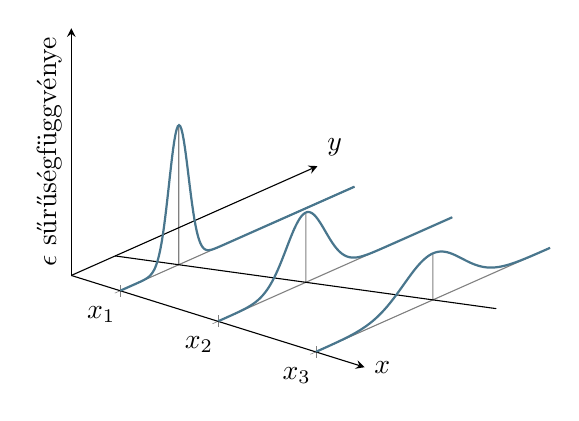
\begin{tikzpicture}[
			declare function={
				normal(\x,\m,\s) = 1/(2*\s*sqrt(pi))*exp(-(\x-\m)^2/(2*\s^2));
			},
			declare function={invgauss(\a,\b) = sqrt(-2*ln(\a))*cos(deg(2*pi*\b));}
			]
			\begin{axis}[
				%no markers,
				domain=0:12,
				zmin=0, zmax=1,
				xmin=0, xmax=3,
				samples=200,
				samples y=0,
				view={40}{30},
				axis lines=middle,
				enlarge y limits=false,
				xtick={0.5,1.5,2.5},
				xmajorgrids,
				xticklabels={},
				ytick=\empty,
				xticklabels={$x_1$, $x_2$, $x_3$},
				ztick=\empty,
				xlabel=$x$, xlabel style={at={(rel axis cs:1,0,0)}, anchor=west},
				ylabel=$y$, ylabel style={at={(rel axis cs:0,1,0)}, anchor=south west},
				zlabel=$\epsilon$ sűrűségfüggvénye, zlabel style={at={(rel axis cs:0,0,0.5)}, rotate=90, anchor=south},
				set layers, mark=cube
				]
				
				\addplot3 [gray!50, only marks, mark=dot, mark layer=like plot, samples=200, domain=0.1:2.9, on layer=axis background] (x, {1.5*(x-0.5)+3+invgauss(rnd,rnd)*x}, 0);
				\addplot3 [samples=2, samples y=0, domain=0:3] (x, {1.5*(x-0.5)+3}, 0);
				\addplot3 [cyan!50!black, thick] (0.5, x, {normal(x, 3, 0.5)});
				\addplot3 [cyan!50!black, thick] (1.5, x, {normal(x, 4.5, 1)});
				\addplot3 [cyan!50!black, thick] (2.5, x, {normal(x, 6, 1.5)});
				
				\pgfplotsextra{
					\begin{pgfonlayer}{axis background}
						\draw [gray, on layer=axis background] (0.5, 3, 0) -- (0.5, 3, {normal(0,0,0.5)}) (0.5,0,0) -- (0.5,12,0)
						(1.5, 4.5, 0) -- (1.5, 4.5, {normal(0,0,1)}) (1.5,0,0) -- (1.5,12,0)
						(2.5, 6, 0) -- (2.5, 6, {normal(0,0,1.5)}) (2.5,0,0) -- (2.5,12,0);
						
					\end{pgfonlayer}
				}
			\end{axis}
		\end{tikzpicture}
	\end{center}
	\subsection{Multikollinearitás}
	Ugyan feltettük, hogy nem létezik tökéletes multikollinearitás, de attól függetlenül valamilyen szintű multikollinearitás mindig elképzelhető a regresszorok között.
	\\
	\\
	Minél nagyobb a multikollinearitás mértéke, annál kevésbé különböznek $\pmb{X}$ oszlopai egymástól, azaz $\pmb{X}$ determinánsa annál kisebb. Emiatt $\pmb{X}^T\pmb{X}$ determinánsa is kisebb lesz, és mivel tetszőleges négyzetes mátrix esetén
	\[
		det(\pmb{A}^{-1}) = det(\pmb{A})^{-1},
	\]
	ezért a paraméterbecslés varianciája képletében $det((\pmb{X}^T\pmb{X})^{-1})$ nagy lesz. Ugyan ez nem egzakt matematikai összefüggés, de intuitíven el lehet képzelni, hogy ez "agresszívebb" $\ebeta$-varianciákat eredményez. Egy másik fontos következmény inkább technikai jellegű, mégpedig hogy a numerikus algoritmus, ami kiszámolja $\pmb{X}^T\pmb{X}$ inverzét, jelentős multikollinearitás mellett pontatlan eredményt fog adni. 
	
	\subsection{A hibavariancia becslése}
	A Gauss-Markov feltevések között szerepelt, hogy a hibatagok regresszorok szerinti feltételes eloszlása normális, egy bizonyos $\pmb{\Sigma}$ variancia-kovariancia mátrixxal. Azt is feltettük, hogy $\pmb{\Sigma}$ alakja
	\[
	\pmb{\Sigma} =
	\begin{bmatrix}
		\sigma^2 & 0 & \dots & 0 \\
		0 & \sigma^2 & \dots & 0 \\
		\vdots & \vdots & \ddots & \vdots \\
		0 & 0 & \dots & \sigma^2
	\end{bmatrix}
	\]
	azaz a mátrix diagonális, és minden diagonálisbeli elem azonosan $\sigma^2$. Felmerül persze a kérdés: Honnan tudjuk, hogy mi ez a $\sigma^2$ variancia? Ennek megoldásához \emph{torzítatlan becslést kell adnunk $\sigma^2$-ra a regresszióból}.
	\\
	\\
	$\sigma^2$ torzítatlan becslése:
	\[
	\widehat{\sigma^2} = \frac{\pmb{e}^T\pmb{e}}{n-p} = \frac{1}{n-p}\sum_{i=1}^{n}{(y_i - \hat{y}_i)^2}
	\]
	ahol $n$ a megfigyelések száma, $p$ pedig a magyarázó változók száma (az interceptet is beleértve). Mivel $p-1$ \emph{valódi magyarázó változónk} van (azaz ami nem konstans, azaz nem $\beta_0$), így a hibavariancia-becslés nevezőjében - a valódi ($\beta_1 \dots \beta_{p-1}$) $p-1$ darab magyarázó változóval - $n-(p-1)-1$ áll.
	
	\section{A $p=2$-es egyváltozós regresszió}
	Nézzük meg, hogy eddig látott paraméterbecslés és becslés-variancia hogy néz ki a legegyszerűbb, egy darab konstans interceptet és egy darab magyarázó változót tartalmazó OLS-el becsült modellben. A modell egyenlete minden $i = 1 \dots n$ megfigyelésre
	\[
	y_i = \beta_0 + \beta_1 x_i + \e_i
	\]
	Az $\pmb{X}$ design mátrixunk most
	\[
	\pmb{X}=
	\begin{bmatrix}
		1 & x_1 \\
		1 & x_2 \\
		\vdots & \vdots \\
		1 & x_n
	\end{bmatrix} \in \mathbb{R}^{n \times 2}
	\]
	lesz, $\ebeta$ paraméterbecslés pedig
	\[
	\ebeta = 
	\left(\begin{bmatrix}
		1 & 1 & \dots & 1 \\
		x_1 & x_2 & \dots & x_n
	\end{bmatrix}
	\begin{bmatrix}
		1 & x_1 \\
		1 & x_2 \\
		\vdots & \vdots \\
		1 & x_n
	\end{bmatrix}\right)^{-1}
	\begin{bmatrix}
		1 & 1 & \dots & 1 \\
		x_1 & x_2 & \dots & x_n
	\end{bmatrix}
	\begin{bmatrix}
		y_1 \\
		y_2 \\
		\vdots \\
		y_n
	\end{bmatrix}
	=
	\begin{bmatrix}
		n & \sum_i{x_i} \\
		\sum_i{x_i} & \sum_i{x_i^2}
	\end{bmatrix}^{-1}
	\begin{bmatrix}
		\sum_i{y_i} \\
		\sum_i{x_i y_i}
	\end{bmatrix}
	\]
	A $2 \times 2$-es mátrixok invertálása könnyen megy:
	\[
	\ebeta = 
	\frac{1}{n\sum_i{x_i^2} - (\sum_i{x_i})^2}
	\begin{bmatrix}
		\sum_i{x_i^2} & -\sum_i{x_i} \\
		-\sum_i{x_i} & n 
	\end{bmatrix}
	\begin{bmatrix}
		\sum_i{y_i} \\
		\sum_i{x_i y_i}
	\end{bmatrix}
	=
	\frac{1}{n\sum_i{x_i^2} - (\sum_i{x_i})^2}
	\begin{bmatrix}
		\sum_i{x_i^2}\sum_i{y_i} - \sum_i{x_i}\sum_i{x_i y_i} \\
		-\sum_i{x_i}\sum_i{y_i} + n\sum_i{x_i y_i}
	\end{bmatrix}
	=
	\]
	\[
	=
	\begin{bmatrix}
		\frac{n(\frac{1}{n}\sum_i{x_i^2}) \cdot n(\frac{1}{n}\sum_i{y_i})-n(\frac{1}{n}\sum_i{x_i}) \cdot n(\frac{1}{n}\sum_i{x_i y_i})}{n^2(\frac{1}{n}\sum_i{x_i^2})-n^2(\frac{1}{n}\sum_i{x_i})^2} \\
		\frac{n^2\frac{1}{n}\sum_i{x_i y_i} - n(\frac{1}{n}\sum_i{x_i}) \cdot n(\frac{1}{n}\sum_i{y_i})}{n^2(\frac{1}{n}\sum_i{x_i^2})-n^2(\frac{1}{n}\sum_i{x_i})^2}
	\end{bmatrix}
	\]
	Az $n$ elemű mintából képzett \emph{mintaátlag} semmi más, mint $\frac{1}{n}\sum_i{x_i}$ illetve $\frac{1}{n}\sum_i{y_i}$, a kovariancia $x$ és $y$ között pedig $\mathbb{E}[xy] - \mathbb{E}[x]\mathbb{E}[y]$, $n$ elemű - a várható értéket torzítatlanul becsülő - mintaátlagokkal ez persze semmi más, mint az \emph{empirikus kovariancia} $ empcov[x,y] = \frac{1}{n}\sum_i{x_i y_i} - (\frac{1}{n}\sum_i{x_i})(\frac{1}{n}\sum_i{y_i})$. $x$ varianciája $\mathbb{E}[x^2] - \mathbb{E}^2[x]$-ként áll elő, $\mathbb{E}[x^2]$ empirikus becslése pedig $\frac{1}{n}\sum_i{x_i^2}$. A vektor mindkét elemében $n^2$-el leosztva látható, hogy a nevezőkben pontosan $x$ mintából számolt varianciája ($empvar$) van, míg a vektor második elemének számlálója pontosan $x$ és $y$ mintából számolt kovarianciája. A vektor első elemének számlálójában $\bar{x^2} \cdot \bar{y} - \bar{x} \cdot \bar{xy}$ áll. Jelölje mostantól a mintából számolt varianciát és kovarianciát $\widehat{Var}$ és $\widehat{Cov}$, ezzel a paraméterbecslés alakja
	\[
	\ebeta =
	\begin{bmatrix}
		\frac{\bar{x^2} \cdot \bar{y} - \bar{x} \cdot \bar{xy}}{\widehat{Var}[x]} \\
		\frac{\widehat{Cov}[x,y]}{\widehat{Var}[x]}
	\end{bmatrix} 
	\]
	Azt kaptuk tehát, hogy a legegyszerűbb egyváltozós regresszió becsült paraméterei
	\[
	\hat{\beta_0} = \frac{\bar{x^2} \cdot \bar{y} - \bar{x} \cdot \bar{xy}}{\widehat{Var}[x]}	
	\]
	\[
	\hat{\beta_1} = \frac{\widehat{Cov}[x,y]}{\widehat{Var}[x]}
	\]
	Sokszor a mintaszámmal normálatlan empirikus kovarianciát és varianciát \emph{$S_{xy}$} és \emph{$S_{xx}$} jelöléssel látják el:
	\[
	S_{xy} = \sum_{i=1}^{n}{(x_i - \bar{x})(y_i - \bar{y})}
	\]
	\[
	S_{xx} = \sum_{i=1}^{n}{(x_i - \bar{x})^2},
	\]
	ezekkel felírva $\beta_1$ becslését:
	\[
	\hat{\beta_1} = \frac{S_{xy}}{S_{xx}}
	\]
	$\beta_0$ becslésének alakja $\beta_1$ ismeretében is kiszámolható, és sokszor ez a módszer sokkal kényelmesebb (már ha ismerjük $\hat{\beta_1}$ értékét):
	\[
	\hat{\beta_0} = \bar{y} - \hat{\beta_1}\bar{x}
	\]
	Ez nem csak intuitívan értelmezhető ("Az átlagos $y$ semmi más, mint az y-tengellyel való metszéspont és $\hat{\beta_1}\bar{x}$ összege"), hanem formálisan is levezethető a modell egyenletéből (meg abból, hogy beláttuk, hogy a paraméterbecslés torzítatlan a feltevéseink mellett, illetve hogy a hibatagok várható értéke $0$):
	\[
	y = \beta_0 + \beta_1 x + \e
	\]
	\[
	\mathbb{E}[y] = \beta_0 + \beta_1\mathbb{E}[x]
	\]
	\[
	\beta_0 = \mathbb{E}[y] - \beta_1 \mathbb{E}[x]
	\]
	A várhatóérték-operátor helyett persze a mintaátlagokkal dolgozva:
	\[
	\beta_0 = \bar{y} - \beta_1 \bar{x}
	\] 
	valóban.
	\subsection{$\ebeta$ varianciája egyváltozós regresszió esetén}
	Láttuk, hogy a paraméterbecslés varianciája az általános esetben
	\[
	Var[\ebeta] = \sigma^2(\pmb{X}^T\pmb{X})^{-1}
	\]
	A már levezetett $p=2$-es design mátrixxal dolgozva:
	\[
	Var[\ebeta] = \sigma^2
	\left(\begin{bmatrix}
		1 & 1 & \dots & 1 \\
		x_1 & x_2 & \dots & x_n
	\end{bmatrix}
	\begin{bmatrix}
		1 & x_1 \\
		1 & x_2 \\
		\vdots & \vdots \\
		1 & x_n
	\end{bmatrix}\right)^{-1}
	=
	\sigma^2
	\frac{1}{n\sum_i{x_i^2} - (\sum_i{x_i})^2}
	\begin{bmatrix}
		\sum_i{x_i^2} & -\sum_i{x_i} \\
		-\sum_i{x_i} & n 
	\end{bmatrix}
	\]
	Használjuk ki az empirikus variancia képletét:
	\[
	n\sum_{i=1}^{n}{x_i^2} - (\sum_{i=1}^{n}{x_i})^2 = n\sum_{i=1}^{n}{(x_i - \bar{x})^2}
	\]
	Innen könnyen látszik, hogy
	\[
	Var[\hat{\beta_0}] = \sigma^2\frac{\sum_{i=1}^{n}{x_i^2}}{n\sum_{i=1}^{n}{(x_i - \bar{x})^2}}
	\]
	\[
	Var[\hat{\beta_1}] = \sigma^2\frac{1}{\sum_{i=1}^{n}{(x_i - \bar{x})^2}}
	\]
	Kimondhatjuk tehát, hogy ahogy $\sigma^2$ nő, úgy nő a paraméterbecslésünk varianciája, avagy \emph{bizonytalansága} is. Hasonlítsuk össze az általános esetben kapott $\ebeta$ variancia képletét $\beta_1$ varianciáéval:
	\[
	\sigma^2(\pmb{X}^T\pmb{X})^{-1}
	\]
	\[
	\sigma^2(\sum_{i=1}^{n}{(x_i - \bar{x})^2})^{-1}
	\]
	A $2 \times 2$-es mátrixszorzást elvégezve tényleg azt kaptuk, hogy az egyváltozós regresszió esetén $S_{xx}$ semmi más, mint az $\pmb{X}^T\pmb{X}$ centralizálatlan regresszor-kovariancia mátrix.
	\\
	\\
	Nagyon fontos - és ezért itt is kihangsúlyozandó - hogy \emph{y varianciája kettő forrásból jön: a regresszorok varianciájából és a regresszorok által nem magyarázott hibavarianciából}. Írjuk ezt az összefüggést fel a mi esetünkben a modellegyenlet segítségével (persze a regresszorok és a hibák korrelálatlansága mellett):
	\[
	Var[\pmb{y}] = \beta_1^2Var[\pmb{x}] + Var[\pmb{\e}] 
	\]
	Itt kihasználtuk, hogy a modell szerint $\beta_0$ konstans, így zérus varianciája van. $Var[\pmb{\e}]$ hibavariancia az a része $y$ varianciájának, amit nem magyaráznak a regresszorok. Ha $Var[\pmb{\e}]$ kicsi, ez annyit jelent, hogy a becsült $\hat{y}$-ok és a tényleges $y$-ok közel vannak egymáshoz, azaz a regresszióval nagyon jól becsülhetjük a valódi $y$ értékeket.
	
	\section{Az $R^2$ mutató}
	Tekintsük az egyváltozós regressziós modellt. Legyen
	\[
	R^2 := \frac{\beta_1^2Var[\pmb{x}]}{Var[\pmb{y}]}
	\]
	az arány, amiben a regresszorok varianciája magyarázza a magyarázott változó teljes varianciáját. $R^2$ $0$ és $1$ közötti szám, minél közelebb van $1$-hez, annál jobban becsülhető $y$ a regresszorokkal. $\beta_1$ becslését beírva adódik:
	\[
	R^2 = \frac{|Cov[\pmb{x},\pmb{y}]|^2}{Var[\pmb{x}]Var[\pmb{y}]}
	\]
	$R^2$ a regresszió "erősségét" mutatja, így a normálatlan empirikus kovarianciákkal és varianciákkal ($S_{xy}$, $S_{xx}$, $S_{yy}$):
	\[
	R^2 = \frac{S^2_{xy}}{S_{xx}S_{yy}}
	\]
	Itt persze $S_{yy} = \sum_i{(y_i - \bar{y})^2}$
	Vezessük be az alábbi jelöléseket:
	\[
	SST = \sum_{i=1}^{n}{(y_i - \bar{y})^2}
	\]
	\[
	SSE = \sum_{i=1}^{n}{(\hat{y}_i - \bar{y})^2}
	\]
	\[
	SSR = \sum_{i=1}^{n}{e_i^2}
	\]
	$SST$ a \emph{Sum of Squares Total}, $SSE$ a \emph{Sum of Squares Explained}, $SSR$ pedig a \emph{Sum of Squares Residual}. Az előbbi varianciafelbontásból könnyen látszik, hogy mivel $SSE$ a regresszorok által magyarázott variancia, $SSR$ pedig a magyarázatlan variancia:
	\[
	SST = SSE + SSR
	\]
	$R^2$-et az előbbihez hasonlóan, csak most az új jelölésekkel felírva:
	\[
	R^2 = \frac{SSE}{SST} = 1- \frac{SSR}{SST}
	\]
	(Az irodalomban néha - zavaró módon - Az $SSE$ a hibák négyzetösszegét jelenti, mint Sum of Squares Error, és az $SSR$ jelenti a magyarázott varianciát, mint Sum of Squares Regression.)
	\section{Kihagyott változó bias - Omitted Variable Bias}
	Tekintsünk egy 
	\[
		y = \beta_0 + \beta_1 x + \beta_2 z + \e
	\]
	lineáris modellt. Ahhoz, hogy létezzen kihagyott változó bias, a kihagyott változó együtthatója nem lehet zérus, illetve a kihagyott változónak \emph{korrelálnia kell} egy másik, regresszióban szereplő magyarázó változóval.
	\\
	\\
	Tegyük fel, hogy kihagyjuk $z$-t a regresszióból:
	\[
		y = \tilde{\beta_0} + \tilde{\beta_1} x + \tilde{\e}
	\]
	és hogy $z$-t $x$ a következőképpen magyarázza:
	\[
		z = \delta_0 + \delta_1 x + \nu
	\]
	Helyettesítsük be a második egyenletet az eredeti teljes egyenletbe:
	\[
		y = (\beta_0 + \beta_2 \delta_0) + (\beta_1 + \beta_2 \delta_1)x + (\e + \beta_2 \nu)
	\]
	Látható, hogy ha ezen a kihagyott változós modellen végeznénk el a regressziós paraméterbecslést, $x$ együtthatójának nem $\beta_1$-et, hanem $\beta_1 + \beta_2 \delta_1$-et kapnánk, ami nyilvánvalóan az eredeti modellel konzisztensen \emph{torzított}. Úgy is gondolhatunk erre, hogy a kihagyott $z$ miatt $x$ becsült együtthatója tartalmazni fogja az indirekt hatást is ($z$-n $x$ hatása $\delta_1$, ezt megszorozva még $y$-n $z$ hatásával).
	\\
	\\
	Mátrixformában az Omitted Variable Bias az alábbi formában szemléltethető. Legyenek
	\[
		\pmb{X} =
		\begin{bmatrix}
		x_1 \\
		x_2 \\
		\vdots \\
		x_n
		\end{bmatrix}, \quad
		\pmb{Z} =
		\begin{bmatrix}
		z_1 \\
		z_2 \\
		\vdots \\
		z_n 
		\end{bmatrix}
	\]
	a regresszorokat tartalmazó vektorok. A $z$-t kihagyó modell design mátrixa pusztán $\pmb{X}$, így az ebből nyert paraméterbecslés
	\[
		\ebeta = (\pmb{X}^T\pmb{X})^{-1}\pmb{X}^T\pmb{y}
	\] 
	Írjuk be $\pmb{y}$ helyére a tényleges, teljes modellből származó alakot:
	\[
		\ebeta = (\pmb{X}^T\pmb{X})^{-1}\pmb{X}^T(\pmb{X}\pmb{\beta} + \pmb{Z}\pmb{\delta} + \pmb{\e}) = \pmb{\beta} + (\pmb{X}^T\pmb{X})^{-1}\pmb{X}^T\pmb{Z}\pmb{\delta} + (\pmb{X}^T\pmb{X})^{-1}\pmb{X}^T\pmb{\e}
	\]
	Mindkét oldalon várható értéket véve, és visszaemlékezve arra, hogy az utolsó tag zérus lesz:
	\[
		\mathbb{E}[\ebeta] = \pmb{\beta} + (\pmb{X}^T\pmb{X})^{-1}\mathbb{E}[\pmb{X}^T\pmb{Z}]\pmb{\delta}
	\]
	ahol látható, hogy a jobb oldal második tagja pontosan a kihagyott $z$ változó miatti torzítás, avagy \emph{bias}.
	
\end{document}
